Un \textbf{Sistema Autónomo (AS)} se define como un conjunto de redes y enrutadores administrados por una única entidad técnica y administrativa. Este concepto es la piedra angular del encaminamiento en Internet, permitiendo dividir la red global en unidades manejables que operan de forma independiente pero coordinada.

\subsection{Características y Responsabilidades del AS}

La existencia de una autoridad única (como un ISP, una universidad o una gran corporación) garantiza que las políticas de enrutamiento dentro de su dominio sean coherentes. El administrador de un AS es responsable de:

\begin{itemize}
	\item Mantener la integridad y convergencia de las rutas internas.
	\item Definir qué información de su red interna será visible para el exterior.
	\item Gestionar las interconexiones con otros Sistemas Autónomos mediante el protocolo BGP.
\end{itemize}

Cada AS tiene total libertad para elegir sus mecanismos de funcionamiento interno. Esto se refleja en la distinción entre protocolos:

\begin{itemize}
	\item \textbf{Protocolos Internos (IGP):} Dentro del AS, se utilizan protocolos como RIP u OSPF para optimizar el tráfico interno basándose en métricas técnicas (distancia, retardo).
	\item \textbf{Ocultamiento de Topología:} El AS se presenta ante el mundo exterior como una "caja negra". Solo se anuncian los prefijos IP alcanzables, ocultando la infraestructura interna para mejorar la seguridad y reducir la carga de procesamiento global.
\end{itemize}

A diferencia del encaminamiento interno, el intercambio entre Sistemas Autónomos se rige por \textbf{políticas comerciales y económicas}. Un AS puede decidir no transitar tráfico de un competidor o preferir una ruta más costosa técnicamente pero más barata económicamente. Para identificar a cada organización en la tabla de rutas global, se utiliza un \textbf{Número de Sistema Autónomo (ASN)} único.

\subsection{Anuncio de Rutas y Perspectiva del Receptor}

El encaminamiento entre sistemas autónomos (mediante BGP) difiere fundamentalmente de los protocolos tradicionales. Mientras que un IGP confía en la topología local, un protocolo de pasarela exterior debe procesar la información antes de anunciarla, actuando como un filtro inteligente. Al suministrar información hacia otros sistemas, un AS debe considerar:

\begin{itemize}
	\item \textbf{Restricciones de Política:} No todas las redes internas son accesibles para usuarios externos. El AS debe filtrar sus anuncios basándose en acuerdos administrativos.
	\item \textbf{Optimización del Próximo Salto:} El AS receptor debe recibir la información de tal manera que pueda dirigir el tráfico de la forma más eficiente posible hacia el destino final.
\end{itemize}  

\subsection{El Salto Extra (\textit{Extra Hop})}

Un aspecto técnico crítico en la configuración de un enrutador de borde es evitar el enrutamiento subóptimo hacia el exterior. Si un enrutador de borde se anuncia ciegamente como el "siguiente salto" para todas las redes de su sistema, podría forzar al tráfico externo a realizar un recorrido innecesario.

\begin{figure}[H]
	\centering
	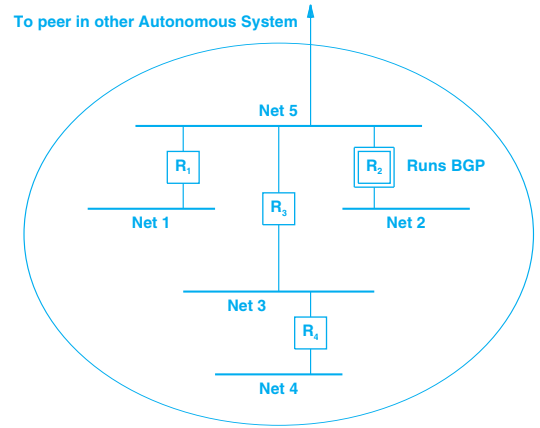
\includegraphics[width=0.5\textwidth]{img/13-10.png}
	\caption{Optimización del siguiente salto para evitar el efecto de salto extra.}
	\label{fig:grafico8}
\end{figure}

Como se ilustra en la Figura \ref{fig:grafico8}, un enrutador de borde (R2) que actúa en nombre de su AS debe informar al vecino el siguiente salto óptimo real. Si la Red 1 es más accesible vía R1, R2 debe indicar a los pares externos que el siguiente salto es R1, no él mismo. Esta transparencia permite que el tráfico entre al AS por el punto más cercano al destino, optimizando los recursos de la red troncal interna.

\subsection{Limitaciones Técnicas del Encaminamiento Exterior}

La restricción fundamental de los protocolos como BGP es que no interpretan métricas de distancia interna. Mientras que un IGP sabe si un enlace es de 1 Gbps o 10 Mbps, BGP solo conoce la \textbf{accesibilidad}. Debido a que la estructura interna de cada AS es privada, un enrutador externo no puede comparar el coste real de dos rutas basándose únicamente en la lista de sistemas atravesados (\textit{AS-PATH}). Esto conlleva varias consecuencias prácticas:

\begin{itemize}
	\item \textbf{Asimetría del Tráfico:} Es común que el tráfico de ida siga una ruta física distinta al de vuelta, ya que cada AS toma decisiones independientes.
	\item \textbf{Falta de Balanceo de Carga Nativo:} BGP suele seleccionar una única ruta preferida, dificultando el reparto equitativo del tráfico entre múltiples enlaces hacia un mismo destino.
	\item \textbf{Predominancia de la Economía:} En el núcleo de Internet, las rutas se eligen por acuerdos de \textit{peering} y tránsito que maximizan ingresos o minimizan costes comerciales, dejando el rendimiento técnico en un segundo plano.
\end{itemize}
